



\documentclass{beamer}
\usepackage[utf8]{inputenc}
\usepackage{url}
\usepackage{algorithm}
\usepackage{algpseudocode}
\usepackage{lmodern}
\usepackage{natbib}
\usepackage{tikz}
\usepackage{physics}
\usepackage{graphicx} % Allows including images
\graphicspath{ {./images/} }
\usepackage{booktabs} % Allows the use of \toprule, \midrule and \bottomrule in tables
\usepackage{tikz}
\usetikzlibrary{arrows.meta}

\usetikzlibrary{mindmap, trees, shadows, shapes, calc, fadings, positioning, decorations.pathreplacing, intersections, shapes, arrows}

%\usetheme{Hannover}
%\usecolortheme{spruce}
% EPIC FAIL
\usetheme{default}
%\usecolortheme{beetle}
\usepackage{graphics}

\usepackage{color}
\definecolor{new_turquoise}{RGB}{40,151,158}%{251,190,94}
\setbeamercolor{title}{fg=new_turquoise}


%\usepackage[colorlinks=true, urlcolor=blue, linkcolor=red]{hyperref}


\makeatletter
\setbeamertemplate{frametitle}{
    \ifbeamercolorempty[bg]{frametitle}{}{\nointerlineskip}%
    \@tempdima=\textwidth%
    \advance\@tempdima by\beamer@leftmargin%
    \advance\@tempdima by\beamer@rightmargin%
    \vspace*{0.8cm} 
    %\hspace*{-3cm}
    %%%%%%%%%%%%% For example insert shift to right
    \begin{beamercolorbox}[sep=0.3cm,center,wd=\the\@tempdima]{frametitle}
        \usebeamerfont{frametitle}%
        \vbox{}\vskip-1ex%
        \if@tempswa\else\csname beamer@ftecenter\endcsname\fi%
        \strut\insertframetitle\strut\par%
        {%
            \ifx\insertframesubtitle\@empty%
            \else%
            {\usebeamerfont{framesubtitle}\usebeamercolor[fg]{framesubtitle}\insertframesubtitle\strut\par}%
            \fi
        }%
        \vskip-1ex%
        \if@tempswa\else\vskip-.3cm\fi% set inside beamercolorbox... evil here...
    \end{beamercolorbox}%
}
\makeatother

\setbeamercolor{frametitle}{fg=new_turquoise}
\setbeamertemplate{itemize item}{\color{new_turquoise}$\blacksquare$}
\setbeamertemplate{itemize subitem}{\color{new_turquoise}$\blacksquare$}


% --- ENUMERATE ITEMS ---
\setbeamertemplate{enumerate item}{\color{new_turquoise}\insertenumlabel}
\setbeamertemplate{enumerate subitem}{\color{new_turquoise}\insertsubenumlabel}

\setbeamertemplate{caption}{\raggedright\insertcaption\par}

% --- COLOR THE TABLE OF CONTENTS ENTRIES ---
\setbeamercolor{section in toc}{fg=new_turquoise}
\setbeamercolor{subsection in toc}{fg=new_turquoise}
\setbeamercolor{subsubsection in toc}{fg=new_turquoise}



\usebackgroundtemplate{
    
\includegraphics[width=\paperwidth,height=\paperheight]{figs/slide-title.jpg}
} 

\title{\fontsize{49}{7.2}{\bf Fundamental Algorithmic Techniques X}}
%\author{JW}
\date{\color{new_turquoise}\today}
%S\titlegraphic{\includegraphics[width=2cm]{figs/jw.png}}

\begin{document}
\frame{\titlepage}
%% SLIDE 1 - INTRO TO THE TEAM
%%%%%%%%%%%%%%%%%%%%%%%%%%%%%%%%%%%%%%%%%%%%%%%%%%%%%

\usebackgroundtemplate{
    
\includegraphics[width=\paperwidth,height=\paperheight]{figs/slide-pages}
} 


\setbeamertemplate{subsection in toc}{
  \color{new_turquoise}$\blacksquare$\color{black}~~\inserttocsubsection
}


% Outline frame
\begin{frame}{Outline}
    \tableofcontents
\end{frame}





\section{Graph Colouring Algorithms}


\begin{frame}{Graph Coloring: Example}
\frametitle{Graph Coloring – Map and Schedule Applications}
\small

\begin{columns}
\begin{column}{0.55\textwidth}
\textbf{Problem}: Assign as {\bf few colors as possible} to vertices so that no two adjacent vertices share the same color.

\vspace{1em}
\textbf{Example:}
\begin{itemize}
\item Vertices: Regions on a map or tasks needing resources
    \item Edges: Conflicts 
\end{itemize}
\textbf{Chromatic Number}: minimum colors needed: \alert{$\chi(G) = 3$} (NP Hard)
\vspace{1em}

\textcolor{new_turquoise}{\bf Real-world use cases:}
\begin{itemize}
    \item Scheduling exams
    \item Register allocation in compilers
    \item Frequency assignment in wireless networks
\end{itemize}
\end{column}

\begin{column}{0.45\textwidth}
\begin{center}
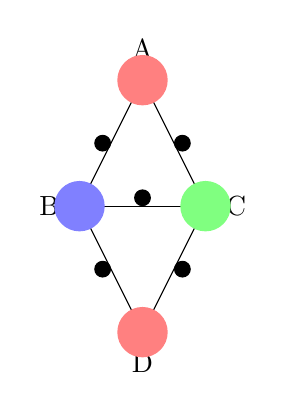
\begin{tikzpicture}[scale=0.8, every node/.style={circle, draw, fill=white, inner sep=2pt}]
    \node[label=above:A] (A) at (0,2) {};
    \node[label=left:B] (B) at (-1,0) {};
    \node[label=right:C] (C) at (1,0) {};
    \node[label=below:D] (D) at (0,-2) {};

    \draw (A) -- (B) node[midway, left, black] {};
    \draw (A) -- (C) node[midway, right, black] {};
    \draw (B) -- (C) node[midway, above, black] {};
    \draw (B) -- (D) node[midway, left, black] {};
    \draw (C) -- (D) node[midway, right, black] {};

    % Color nodes
    \fill[red!50] (A) circle (0.4cm);
    \fill[blue!50] (B) circle (0.4cm);
    \fill[green!50] (C) circle (0.4cm);
    \fill[red!50] (D) circle (0.4cm);
\end{tikzpicture}
\end{center}
\footnotesize\textit{A 3-coloring: A,D=red; B=blue; C=green}
\end{column}
\end{columns}
\end{frame}


\begin{frame}{Nice examples of graph colouring problems}
\begin{columns}
\begin{column}{0.48\textwidth}
\begin{center}
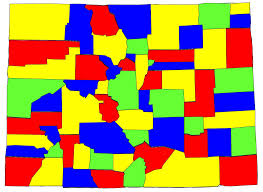
\includegraphics[width=\linewidth]{Algos_figs/graphcoulouringpbm1.jpeg}
\end{center}
\end{column}
\begin{column}{0.48\textwidth}
\begin{center}
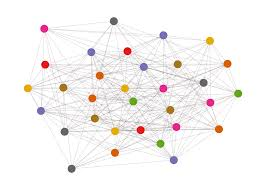
\includegraphics[width=\linewidth]{Algos_figs/graphcoulouringpbm2.jpeg}
\end{center}
\end{column}
\end{columns}
\end{frame}


\begin{frame}{Bipartite Graphs \& Graph Coloring}

\textcolor{new_turquoise}{\bf Bipartite Graph}\\
A graph whose vertices can be divided into two disjoint sets $U$ and $V$, such that every edge connects a vertex in $U$ to one in $V$.\\[0.1cm]
Equivalently: 2-colorable — no two adjacent vertices share the same color.

\vspace{0.3cm}
\textcolor{new_turquoise}{\bf When is a graph bipartite?}\\
$\iff$ No odd-length cycles.\\
Example: Trees, even cycles, hypercubes.

\vspace{0.4cm}
\textcolor{new_turquoise}{\bf Beyond Two Colors: Four Color Theorem}\\
Every planar graph (or map) is 4-colorable — no two adjacent regions need more than four colors.\\[0.1cm]
\fbox{\small First major theorem proven with computer assistance (1976, Appel \& Haken)}

\end{frame}



\begin{frame}{Graph Coloring Algorithm: Greedy Coloring}
\small

\begin{columns}

% Left column: Algorithm and key properties
\begin{column}{0.55\textwidth}
\textbf{Algorithm (Greedy Coloring)}:
\begin{enumerate}
    \item Order vertices: $v_1, v_2, \dots, v_n$
    \item For each $v_i$ in order:
    \item[] $\quad$ Assign the smallest color not used by its already-colored neighbors.
\end{enumerate}

\textbf{Key Properties}:
\footnotesize
\begin{itemize}
\item Time complexity: $O(V + E)$
    \item Not optimal — may use $> \chi(G)$ colors
    \item Performance depends on vertex ordering
    \item Worst case: $\chi(G) + 1$ colors %($\Delta = \max \deg$)
    \item Heuristics: DSATUR, Largest First, Smallest Last
\end{itemize}
\end{column}

% Right column: Example table and image placeholder
\begin{column}{0.5\textwidth}
\begin{center}
\footnotesize
\begin{tabular}{c|c|c}
Vertex & Neighbors' Colors & Color Assigned \\
\hline
$v_1$ & — & \textcolor{red}{1} \\
$v_2$ & \{1\} & \textcolor{blue}{2} \\
$v_3$ & \{1,2\} & \textcolor{green}{3} \\
$v_4$ & \{2,3\} & \textcolor{red}{1} \\
\end{tabular}
\end{center}

%\vspace{1em}
%\begin{center}
%\includegraphics[width=0.9\linewidth]{Algos_figs/}
%\end{center}
%\footnotesize\textit{Example run of greedy coloring}
\end{column}

\end{columns}

\end{frame}





\begin{frame}{Flood Fill: More Than Just a Paint Tool}

\textcolor{new_turquoise}{\bf It’s Graph Traversal on a Grid}\\
Each pixel is a node; edges connect to 4 neighbors.\\
Flood fill = find connected component of same color.

\vspace{0.3cm}
\textcolor{new_turquoise}{\bf Why Queue? Avoid Stack Overflow}\\
Recursive DFS crashes on large regions (e.g., 1M pixels).\\
Queue → iterative BFS → safe, predictable memory use.

\vspace{0.3cm}
\textcolor{new_turquoise}{\bf BFS vs DFS: Shape Matters!}
\begin{itemize}

\item \textbf{BFS (Queue)}: Circular, even fill — \textit{used in Photoshop}
    \item \textbf{DFS (Stack)}: Jagged, spiky fill — \textit{faster on small areas}
\end{itemize}
\vspace{0.3cm}
\textcolor{new_turquoise}{\bf Applications}
\begin{itemize}
    \item Medical imaging: Segment tumors or organs
    \item Computer vision: Object detection via region growing
    \item Game engines: Territory control, pathfinding
\end{itemize}
\end{frame}





\section{Shortest Paths}




\begin{frame}{Dijkstra's Algorithm}
\small

\textbf{Goal:} Find shortest paths from a source node to all other nodes in a weighted graph (non-negative weights).

\vspace{1em}

\textbf{Simple Steps:}

\begin{enumerate}
    \item Set distance to source = 0. Set all other distances to $\infty$. Mark all nodes unvisited.
    \item While there are unvisited nodes:
    \item Choose the unvisited node with the smallest known distance.
        \item For each neighbor of that node:
        \begin{itemize}
            \item Add the edge weight to the current node’s distance.
            \item If this gives a shorter path to the neighbor, update its distance.
        \item Mark the current node as visited.
    \end{itemize}
\end{enumerate}

\vspace{1em}

\textbf{Key idea:} Greedily expand the closest unvisited node — guarantees optimal paths.

\end{frame}

\begin{frame}{Dijkstra's Algorithm: Step-by-Step Execution}
\begin{center}
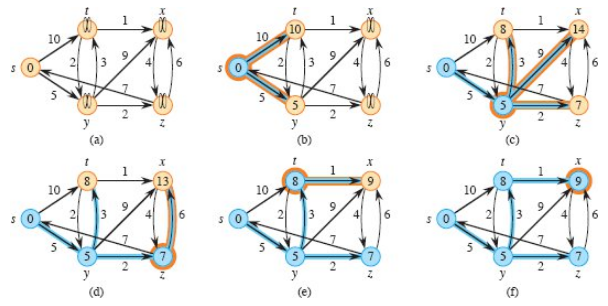
\includegraphics[width=0.95\textwidth]{Algos_figs/Dijskra.png}
\end{center}
\begin{center}
\footnotesize\textit{Dijkstra's algorithm: shortest path tree built step by step}
\end{center}
\end{frame}



\begin{frame}{Bellman-Ford: Shortest Paths with Negative Weights}
\tiny
\textcolor{new_turquoise}{\bf Why Bellman-Ford?}

\begin{itemize}
\item Handles \textbf{negative edge weights} (unlike Dijkstra)
    \item Detects \textbf{negative cycles} — paths with $-\infty$ weight
    \item Works on graphs where Dijkstra fails due to negative edges
\end{itemize}

\vspace{0.3cm}
\textcolor{new_turquoise}{\bf Key Algorithmic Ideas}
\begin{itemize}
\item Initialize all distances to $\infty$, except source to $0$
    \item \textbf{Relaxation}: If $\text{dist}[u] + \text{wt} < \text{dist}[v]$, update $\text{dist}[v]$
    \item Repeat relaxation for \textbf{at most $V-1$ iterations} (tree property and so not sensitive to neg. paths)
    \item Run $V$-th iteration to detect negative cycles
\end{itemize}
\vspace{0.3cm}
\textcolor{new_turquoise}{\bf Complexity}
\begin{enumerate}
\item \textbf{Time}: $O(VE)$ — $V-1$ passes, $E$ edges each
    \item \textbf{Space}: $O(V)$ — distance array only
    \item \textbf{vs Dijkstra}: $O(E \log V)$, but no negative edges allowed
\end{enumerate}
\vspace{0.2cm}
\textcolor{new_turquoise}{\bf Pseudocode}
\begin{align*}
&\text{for } i = 1 \text{ to } V-1: \\
&\quad \text{for each edge } (u,v) \text{ with weight } w: \\
&\quad\quad \text{if } \text{dist}[u] + w < \text{dist}[v]: \\
&\quad\quad\quad \text{dist}[v] = \text{dist}[u] + w \\
&\text{for each edge } (u,v) \text{ with weight } w: \quad \text{// Negative cycle check} \\
&\quad \text{if } \text{dist}[u] + w < \text{dist}[v]: \text{ return ``Negative cycle detected''}
\end{align*}
\end{frame}


\begin{frame}{Bellman-Ford: Example Execution}
\tiny

\textcolor{new_turquoise}{\bf Example Illustration}

\begin{center}
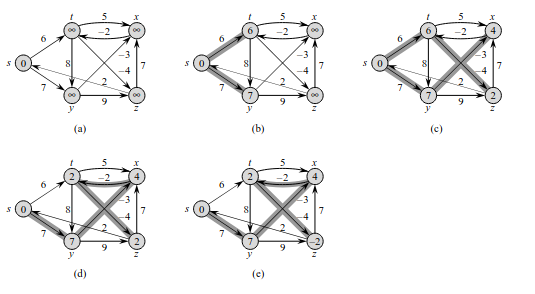
\includegraphics[width=0.75\textwidth]{Algos_figs/bellman-ford.png}
\end{center}

\vspace{0.3cm}

\textcolor{new_turquoise}{\bf What is happening?}

\begin{itemize}
    \item The algorithm repeatedly \textbf{relaxes all edges} in the graph
    \item Each iteration propagates shorter distances further from the source
    \item After $k$ iterations, all shortest paths using at most $k$ edges are found
    \item After $V-1$ iterations, all shortest paths are guaranteed to be correct
    \item A final pass checks for further improvements → detects \textbf{negative cycles}
\end{itemize}

\vspace{0.2cm}

\textcolor{new_turquoise}{\bf Intuition}

\begin{itemize}
    \item Think of distances as “waves” spreading from the source
    \item Negative edges can pull distances down, but only finitely unless a cycle exists
\end{itemize}

\end{frame}


\section{Flow Networks}

% Slide 1: Flow Network
\begin{frame}{Flow Network}
A \textcolor{new_turquoise}{\bf Flow Network} is a directed graph \( G = (V, E) \) with:
\begin{itemize}

\item A \textbf{source} \( s \in V \) and a \textbf{sink} \( t \in V \)
    \item A \textbf{capacity function} \( c : E \to \mathbb{R}_{\geq 0} \)
    \item A \textbf{flow function} \( f : E \to \mathbb{R}_{\geq 0} \) satisfying:
    \begin{enumerate}
        \item \textbf{Capacity constraint: } \( 0 \leq f(u,v) \leq c(u,v) \)
        \item \textbf{Flow conservation: } \( \sum_{w} f(w,u) = \sum_{w} f(u,w) \) for all \( u \neq s,t \)
    \end{enumerate}
\end{itemize}
\textbf{Value of flow: } \( |f| = \sum_{v} f(s,v) - \sum_{v} f(v,s) \)

\vspace{0.5em}
	Goal: Find a flow of {\bf maximum value} from \( s \) to \( t \).
\end{frame}


\begin{frame}{Max-Flow Min-Cut Theorem \& Duality}
\textbf{Cut:} A partition \( (S, T) \) of \( V \) with \( s \in S \), \( t \in T \).  
\textbf{Capacity of cut: } \( c(S,T) = \sum_{u \in S,\, v \in T} c(u,v) \)

\begin{block}{\textcolor{new_turquoise}{Max-Flow Min-Cut Theorem}}
\[
\max_{f} |f| \;=\; \min_{(S,T)} c(S,T)
\]
The maximum flow value equals the minimum cut capacity.
\end{block}

\begin{block}{\textcolor{new_turquoise}{LP Duality Perspective}}
\begin{itemize}

\item Max-flow is a linear program.
    \item The dual of the max-flow LP corresponds to a fractional min-cut.
    \item Strong duality \(\Rightarrow\) integral optimal solutions coincide.
    
\end{itemize}
\end{block}

\[
\text{Primal (Max-Flow)} \quad \leftrightarrow \quad \text{Dual (Min-Cut)}
\]
\end{frame}

\end{document}

